\documentclass[tikz]{standalone}

\usetikzlibrary{positioning}
\usepackage{xfrac}
\tikzstyle{node}=[draw=#1,fill=#1!20]

\newcommand{\vertex}[6]{\node[shape=circle,fill=black, scale=0.5,label=#1:{#2},label=#5:{\tiny\texttt{\color{blue}#6}},#4] (#3)  {};}
\newcommand{\myedge}[4]{ \draw[->] (#1) edge node[#2] {#3} (#4);}
\newcommand{\myedger}[4]{ \draw[->] (#1) edge [bend right] node[#2] {#3} (#4);}
\newcommand{\myedgel}[4]{ \draw[->] (#1) edge [bend left] node[#2] {#3} (#4);}
\usetikzlibrary{automata}
\tikzset{
	initial text=\(\ast\),
}


\begin{document}
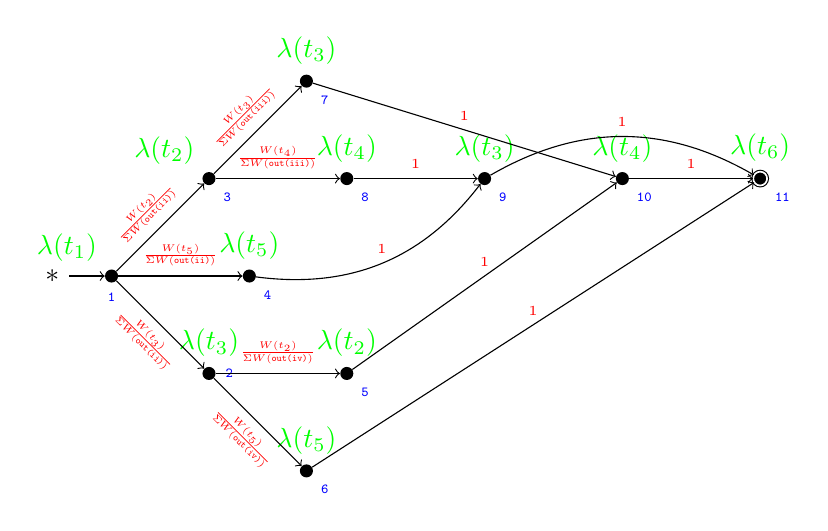
\begin{tikzpicture}[align=center,node distance=3.5cm]
    % equidistant points and arc
    \vertex{above left}{$\color{green}\lambda(t_1)$}{a}{initial}{below}{1}
    
    \vertex{above}{$\color{green}\lambda(t_3)$}{b1}{below right of=a}{right}{2}
    \myedge{a}{midway,below,rotate=315}{\scalebox{.7}{$\scriptscriptstyle{\color{red}\frac{W(t_3)}{\Sigma W(\texttt{out(ii)})}}$}}{b1}
    
    \vertex{above left}{$\color{green}\lambda(t_2)$}{b2}{above right of=a}{below right}{3}
    \myedge{a}{midway, above, rotate=45 }{\scalebox{.7}{$\scriptscriptstyle{\color{red}\frac{W(t_2)}{\Sigma W(\texttt{out(ii)})}}$}}{b2}
    \vertex{above}{$\color{green}\lambda(t_5)$}{b3}{right of=a}{below right}{4}
    \myedge{a}{midway, above }{\scalebox{.7}{$\scriptscriptstyle{\color{red}\frac{W(t_5)}{\Sigma W(\texttt{out(ii)})}}$}}{b3}
    
    
    \vertex{above}{$\color{green}\lambda(t_2)$}{c1}{ right of=b1}{below right}{5}
    \myedge{b1}{midway, above}{\scalebox{.7}{$\scriptscriptstyle{\color{red}\frac{W(t_2)}{\Sigma W(\texttt{out(iv)})}}$}}{c1}
    \vertex{above}{$\color{green}\lambda(t_5)$}{c2}{below right of=b1}{below right}{6}
    \myedge{b1}{midway, below,rotate=315 }{\scalebox{.7}{$\scriptscriptstyle{\color{red}\frac{W(t_5)}{\Sigma W(\texttt{out(iv)})}}$}}{c2}
    
   
   \node[] (bogus1) [right=40pt of b2] {};
    \vertex{above}{$\color{green}\lambda(t_3)$}{d1}{above right of=b2}{below right}{7}
    \myedge{b2}{above,rotate=45 }{\scalebox{.7}{$\scriptscriptstyle{\color{red}\frac{W(t_3)}{\Sigma W(\texttt{out(iii)})}}$}}{d1}
    \vertex{above}{$\color{green}\lambda(t_4)$}{d2}{right of=b2}{below right}{8}
    \myedge{b2}{midway, above}{\scalebox{.7}{$\scriptscriptstyle{\color{red}\frac{W(t_4)}{\Sigma W(\texttt{out(iii)})}}$}}{d2}
    
    
    \vertex{above}{$\color{green}\lambda(t_3)$}{t3}{ right of=d2}{below right}{9}
    \myedge{d2}{midway, above}{{$\scriptscriptstyle{\color{red}1}$}}{t3}
    \myedger{b3}{midway, above}{{$\scriptscriptstyle{\color{red}1}$}}{t3}
        
        
    \vertex{above}{$\color{green}\lambda(t_4)$}{t4}{ right of=t3}{below right}{10}
    \myedge{c1}{midway, above}{{$\scriptscriptstyle{\color{red}1}$}}{t4}
    \myedge{d1}{midway, above}{{$\scriptscriptstyle{\color{red}1}$}}{t4}
        
        
    \vertex{above}{$\color{green}\lambda(t_6)$}{t6}{ right of=t4,accepting,state,scale=0.4}{below right}{11}
    
   
    \myedge{c2}{midway, above}{{$\scriptscriptstyle{\color{red}1}$}}{t6}
    \myedge{t4}{midway, above}{{$\scriptscriptstyle{\color{red}1}$}}{t6}
    \myedgel{t3}{midway, above}{{$\scriptscriptstyle{\color{red}1}$}}{t6}
    
    %\vertex{above}{$\color{green}t_6$}{f}{right of=d2}{below right}{20}
    
%    \vertex{above}{$\color{green}\varepsilon_1$}{s}{initial}{right}{1}
%    \vertex{above}{$\color{green}a$}{b1}{above right of=s}{below right}{2}
%    \vertex{above}{$\color{green}c$}{b2}{below right of=s}{below right}{3}
%    \vertex{above}{$\color{green}\varepsilon_2$}{e2}{right of=b2}{below right}{4}
%    \vertex{above}{$\color{green}b$}{b}{right of=e2}{below right}{5}
%    \vertex{above}{$\color{green}\varepsilon_3$}{f}{right of=b1,accepting,state,scale=0.4}{below right}{6}
%    
%    
%    \myedge{s}{above}{$\scriptscriptstyle{\color{red}p_1}$}{b1}
%    \myedge{s}{above}{$\scriptscriptstyle{\color{red}p_2}$}{b2}
%    \myedge{b2}{above}{$\scriptscriptstyle{\color{red}1}$}{e2}
%    \myedge{e2}{above}{$\scriptscriptstyle{\color{red}p_4}$}{b1}
%    \myedge{e2}{above}{$\scriptscriptstyle{\color{red}p_5}$}{b}
%    \myedge{b}{right}{$\scriptscriptstyle{\color{red}1}$}{f}
%    \myedge{b1}{above}{$\scriptscriptstyle{\color{red}p_6}$}{f}
    
%    \draw[->,shorten >=1pt] (b1) edge [in=135,out=45,loop,looseness=20] node [above] {$\scriptscriptstyle{\color{red}p_3}$} (b1);
\end{tikzpicture}

\end{document}
